\chapter{Aplicação exemplar com arquitetura de microsserviços}\label{chapter-aplicacao}

\chapterprecis{Este capítulo apresenta a aplicação exemplar com arquitetura de microsserviços desenvolvida.}\index{sinopse de capítulo}


A aplicação desenvolvida trata-se de um sistema web de \emph{E-commerce}. Nela, um cliente da loja pode buscar e comprar produtos, enquanto um administrador pode gerenciar produtos e usuários cadastrados, tudo a partir de uma interface de usuário em um navegador.
O código fonte está disponível no repositório do GitHub com link \url{https://github.com/Jp9910/microservices_project}.
% os diagramas de classes, pacotes e componentes podem ser vistos na \autoref{figura-diagrama-de-classes}, \autoref{figura-diagrama-de-pacotes} e \autoref{figura-diagrama-de-componentes}, respectivamente.

\section{A aplicação e a divisão em microsserviços}

A composição da aplicação pode ser vista no diagrama de componentes da aplicação, na \autoref{figura-diagrama-de-componentes}. Já a divisão dos microsserviços, em formato de pacotes, pode ser vista no diagrama de pacotes da aplicação, na \autoref{figura-diagrama-de-pacotes}, que fornece mais detalhes sobre a estrutura interna de cada microsserviço e como eles se conectam. Ademais, as responsabilidades de cada microsserviço são explicadas a seguir

\begin{figure}[htb]
	\caption{\label{figura-diagrama-de-componentes}Diagrama de componentes da aplicação exemplar}
	\begin{center}
	    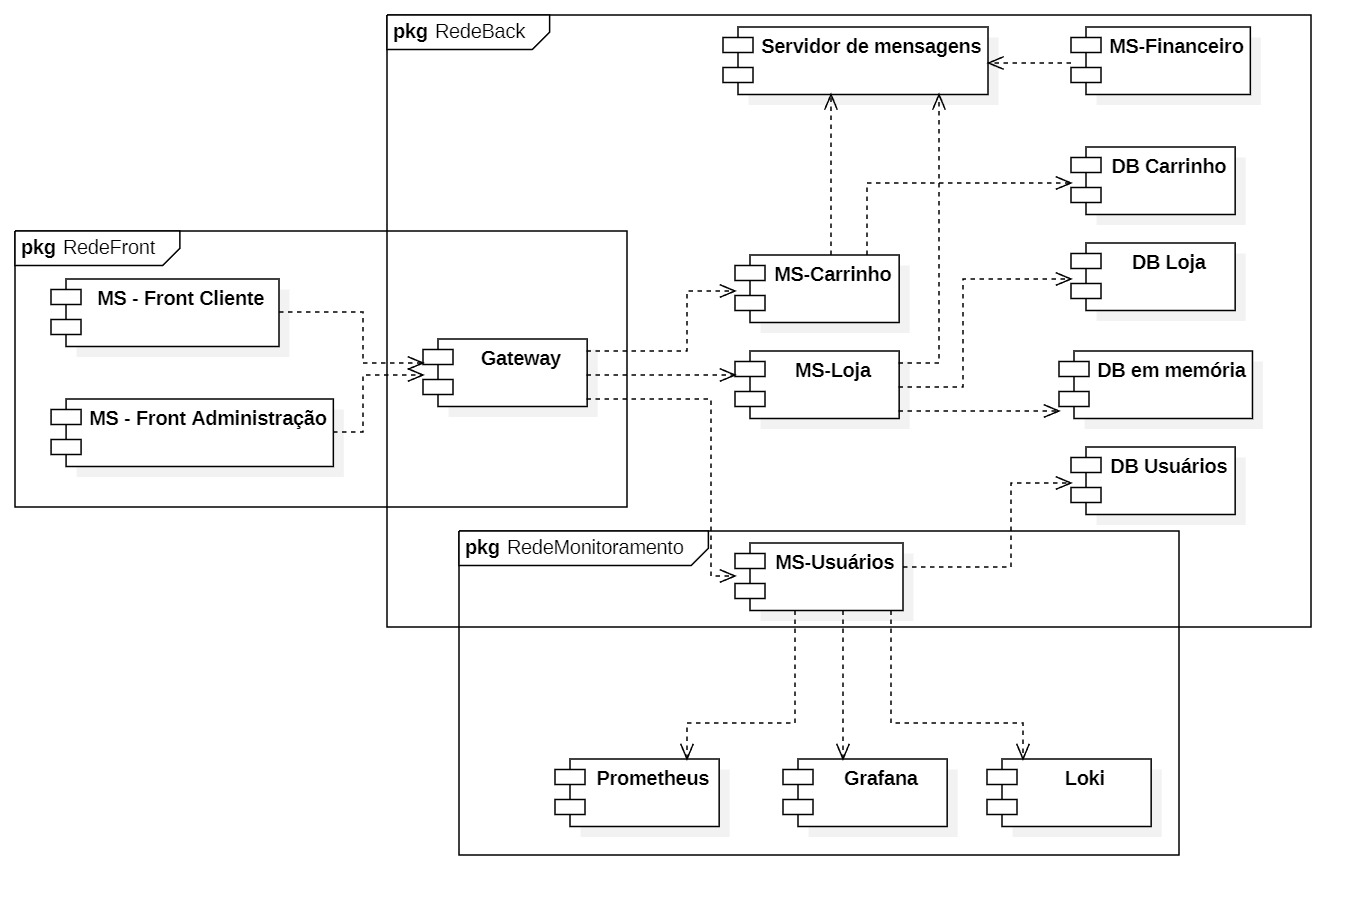
\includegraphics[scale=0.27]{Diagramas/imagens/Componentes-Redes.jpg}
	\end{center}
	\legend{Fonte: Autor}
\end{figure}

\begin{figure}[htb]
	\caption{\label{figura-diagrama-de-pacotes}Diagrama de pacotes da aplicação exemplar}
	\begin{center}
	    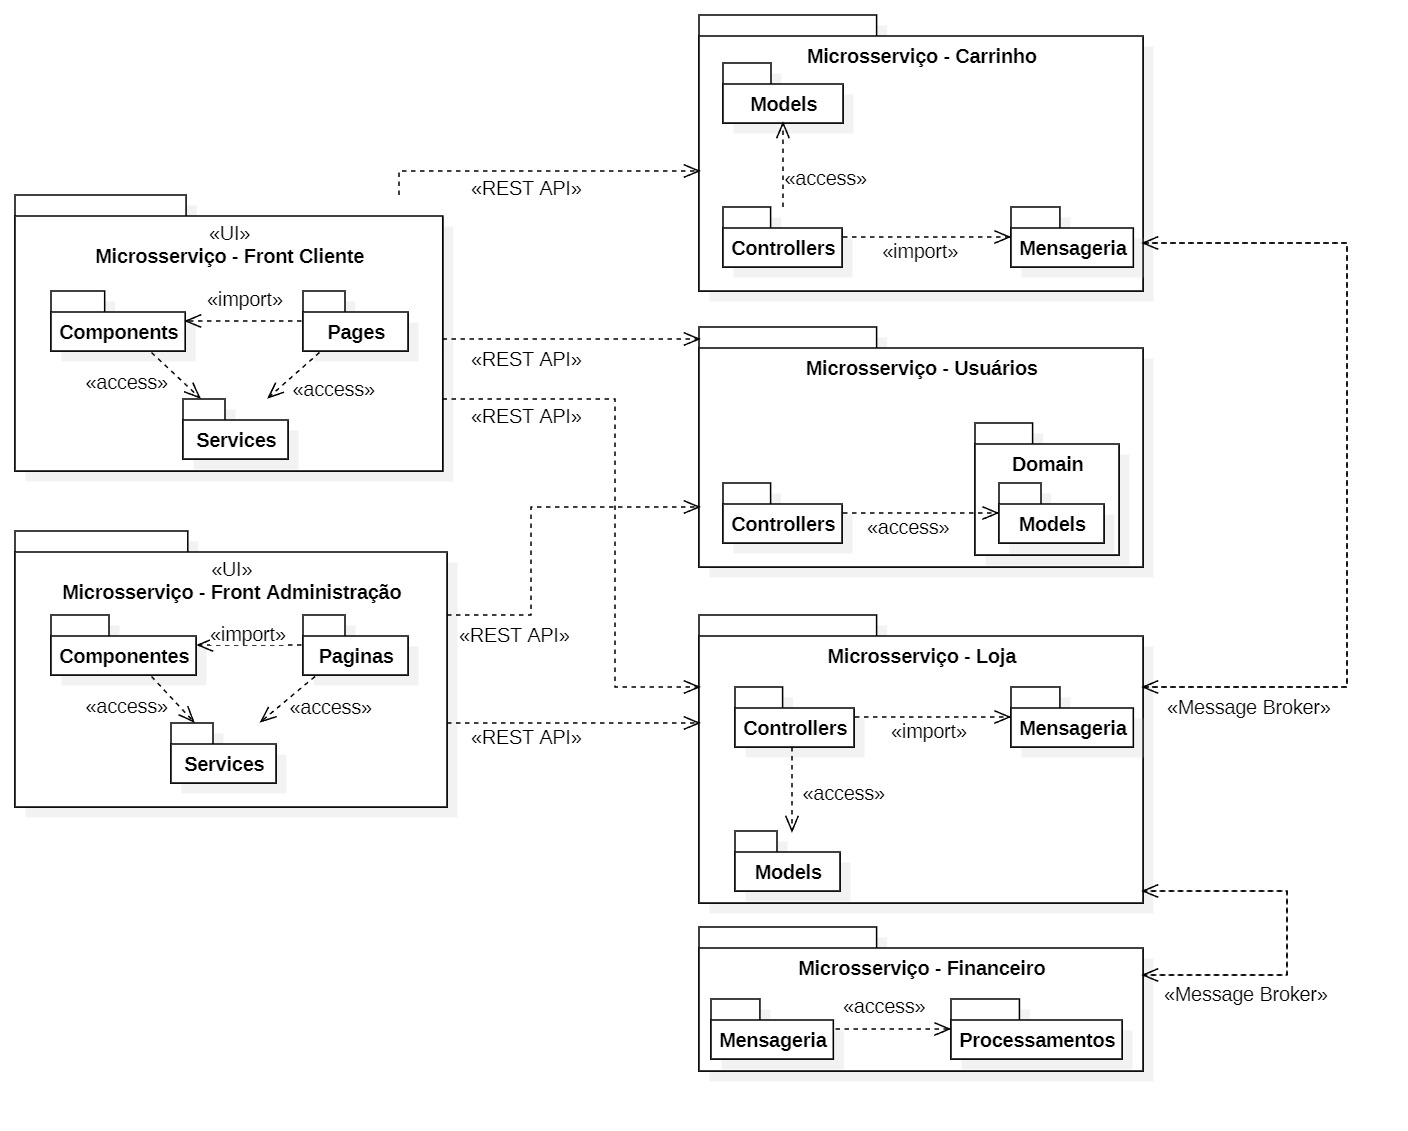
\includegraphics[scale=0.27]{Diagramas/imagens/Pacotes.jpg}
	\end{center}
	\legend{Fonte: Autor}
\end{figure}

\subsubsection*{Microsserviço de loja}
Esse é um microsserviço de negócio que trata do armazenamento e lógica de negócios relacionada a produtos e pedidos.

\subsubsection*{Microsserviço de carrinho}
Esse é um microsserviço de negócio que trata do armazenamento e lógica de negócios relacionada ao carrinho.

\subsubsection*{Microsserviço de usuários}
Esse é um microsserviço de negócio que trata do armazenamento e lógica de negócios relacionada aos usuários do sistema, incluindo autenticação.

\subsubsection*{Microsserviço financeiro}
Esse é um microsserviço de negócio que trata apenas do processamento fictício do pagamento de um pedido.

\subsubsection*{Microsserviço de clientes}
Esse é um microsserviço de ponta que clientes da loja podem acessar para realizar todas as operações relevantes a eles a partir de uma interface de usuário, tal como ver e buscar produtos, adicionar produtos ao carrinho e realizar um pedido a partir de um carrinho.

\subsubsection*{Microsserviço de administração}
Esse é um microsserviço de ponta que administradores da loja podem acessar para realizar todas as operações relevantes a eles a partir de uma interface de usuário, tal como adicionar e alterar produtos do catálogo da loja e adicionar ou alterar usuários do sistema.

% Para dividir os microsserviços e determinar seus limites, foram usados conceitos do ddd para determinar os limites de cada microsserviço...

Para a divisão do sistema em torno dos domínios de negócio, foram aplicados alguns princípios do \hyperref[section-ddd]{\emph{Domain-Driven Design}}, sendo inicialmente identificados os seguintes contextos limitados (\emph{bounded contexts}): Catálogo, Carrinho, Pedidos, Pagamentos, \emph{Marketing} e Usuários. Cada um desses poderia compor um microsserviço, entretanto, para não criar um sistema complexo demais para ser desenvolvido por apenas uma pessoa em pouco tempo, alguns desses foram mesclados em um só ou descartados. \emph{Marketing} parecia ser o contexto menos relevante para o funcionamento adequado do sistema, portanto foi descartado. Também foi decidido que o contexto de pedidos poderia ser mesclado ou com o contexto de produtos ou com o de carrinho por serem relacionados.

% que os contextos de pedidos e produtos seriam mesclados para serem responsabilidade apenas do microsserviço de loja, mas essa não foi uma decisão fácil.

Determinar qual desses dois contextos seria o mais apropriado para a mescla não foi fácil, e certamente terá implicações futuras na manutenção do sistema. No fim, foi decidido que o contexto de pedidos seria mesclado com o contexto de catálogo, assim sendo responsabilidade do microsserviço de loja, pois pedidos são naturalmente relacionados com produtos e necessitam de alta consistência por envolver múltiplas operações, assim tornando o banco de dados relacional, que foi o escolhido para o armazenamento dos produtos, mais apropriado para o caso, em contraste com o banco de dados NoSQL, que foi o escolhido para armazenamento dos carrinhos. Essa decisão está refletida no diagrama de classes da aplicação, apresentado na \autoref{figura-diagrama-de-classes}, onde podem ser vistos as classes, controladores e fronteiras da aplicação e suas associações.

\begin{figure}[htb]
	\caption{\label{figura-diagrama-de-classes}Diagrama de classes da aplicação exemplar}
	\begin{center}
	    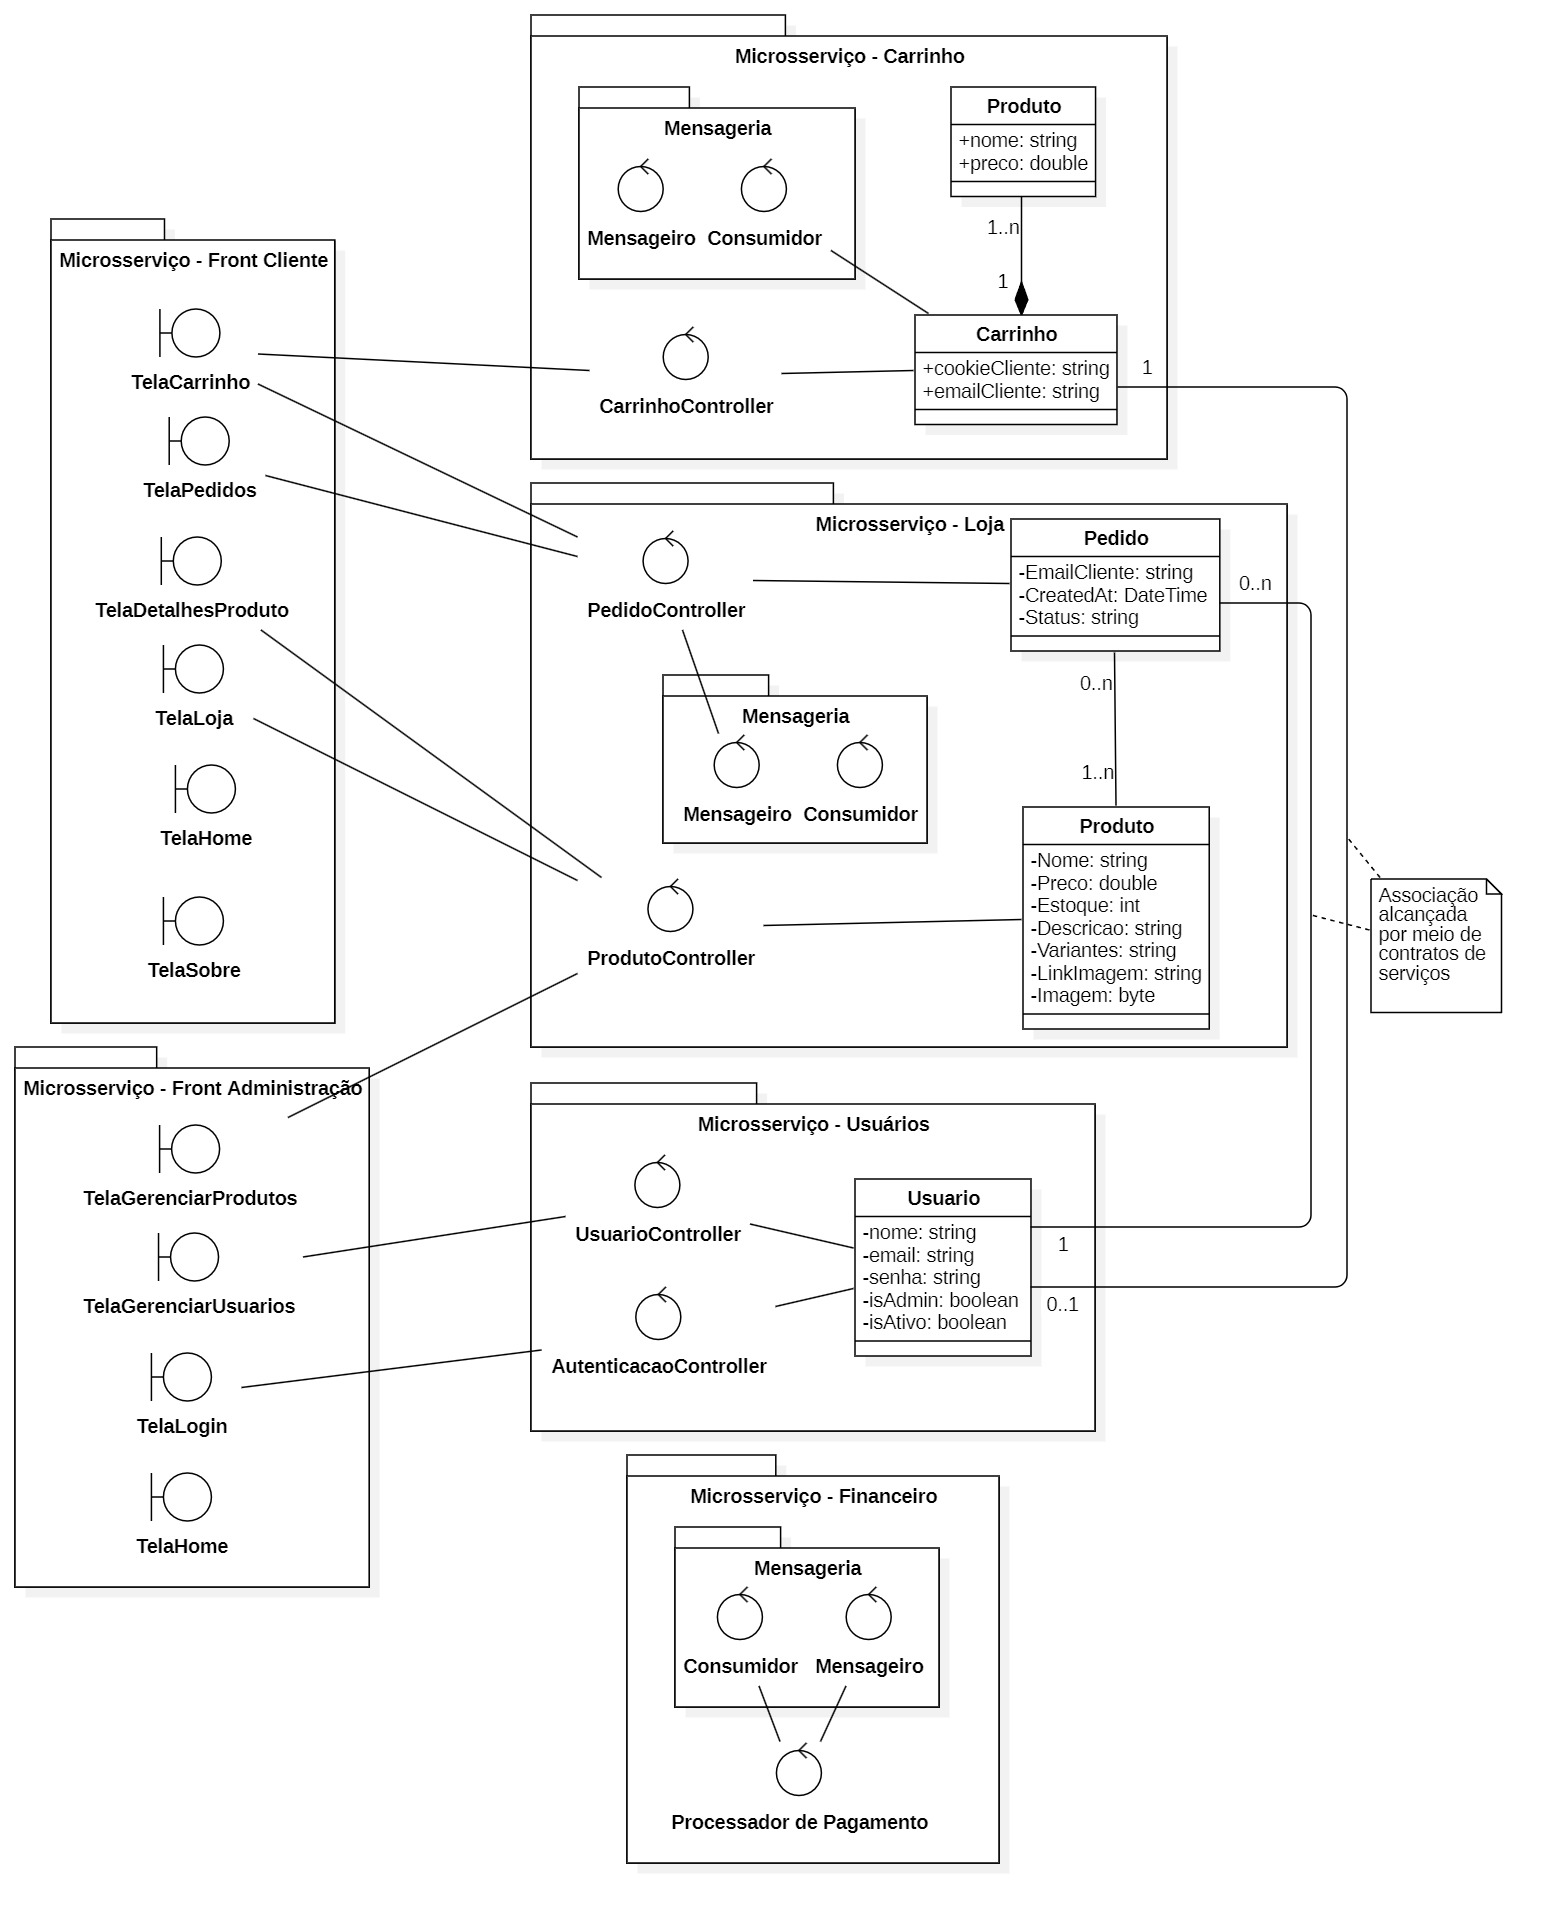
\includegraphics[scale=0.25]{Diagramas/imagens/Classes.jpg}
	\end{center}
	\legend{Fonte: Autor}
\end{figure}

Além disso, para favorecer uma linguagem ubíqua, os nomes das representações das entidades em cada microsserviço foram definidos de acordo com o domínio em questão. Um usuário, por exemplo, é chamado de usuário (do sistema) no microsserviço de usuários, porém no microsserviço de loja, ele é chamado de cliente.

Por fim, também é mostrado a seguir o diagrama de sequência de um dos casos de uso da aplicação. Apesar da aplicação dispor de diversos casos de uso, foi escolhido apenas o mais complexo para ser mostrado, pois o foco não é explorar a lógica de negócios representada; e sim ilustrar como geralmente acontecem a comunicação e o fluxo de mensagens em uma arquitetura de microsserviços como resultado da ação de um usuário. Trata-se do diagrama de sequência do caso de uso de realizar uma compra no carrinho, que pode ser visto na \autoref{figura-diagrama-de-sequencia}

\begin{figure}[htb]
	\caption{\label{figura-diagrama-de-sequencia}Diagrama de sequência do caso de uso de realizar uma compra no carrinho}
	\begin{center}
	    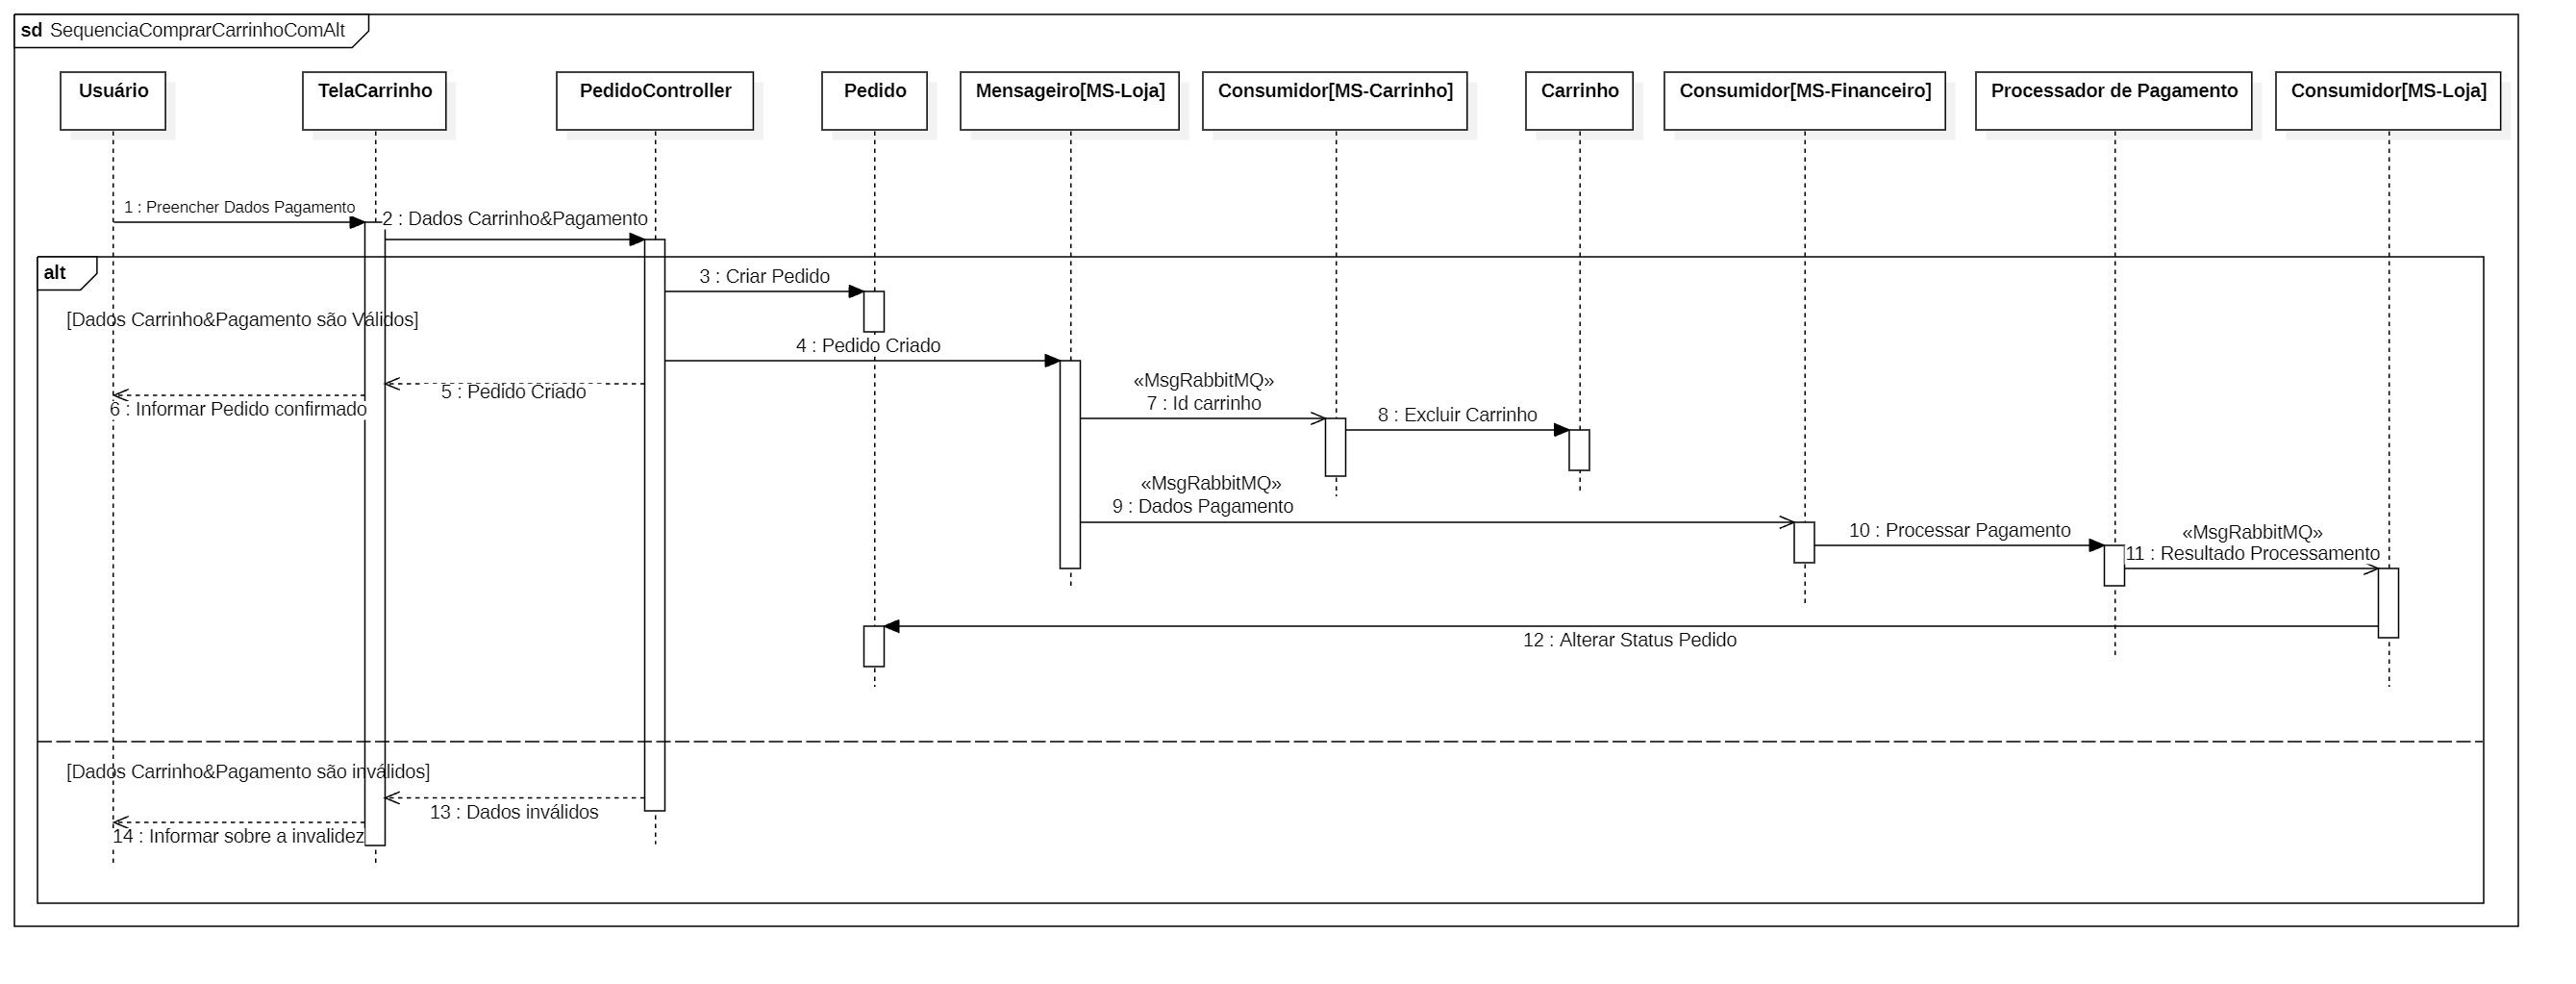
\includegraphics[scale=0.16]{Diagramas/imagens/SequenciaComprarCarrinhoComAlt.jpg}
	\end{center}
	\legend{Fonte: Autor}
\end{figure}

% Em especial houve uma dúvida muito grande quanto a qual microsserviço será responsável pela lógica de negócios dos pedidos e seu armazenamento. Foram considerados o microsserviço de carrinho (que viraria o microsserviço de pedidos) ou o microsserviço de loja (que sem os pedidos viraria o microsserviço de catálogo). No fim decidi implementar no microsserviço de loja porque...

% Além disso, a aplicação dos conceitos de Entidades, Value Objects, Agregados e Serviços de Domínio possibilitou uma organização mais robusta e coesa da lógica de negócio. Cada microsserviço foi projetado para encapsular um contexto bem delimitado, onde a integridade dos dados era mantida por meio de contratos claros e limites bem definidos. Dessa forma, os princípios do Domain-Driven Design contribuíram para que os microsserviços operassem de forma autônoma, escalável e facilmente adaptável às evoluções e demandas do mercado.

% Além disso, na mesma aplicação, optei por implementar a arquitetura CLEAN, o que fortaleceu a independência entre os componentes e camadas do sistema. Ao aplicar essa arquitetura, pude isolar a lógica de domínio das dependências externas, como frameworks, bancos de dados e interfaces de usuário. Essa separação resultou em um design mais robusto, onde a lógica de negócio permanece centralizada e facilmente testável, permitindo a evolução contínua dos microserviços sem o risco de efeitos colaterais indesejados.

\section{Práticas, ferramentas e padrões usados}

\subsection{\emph{Frameworks} e linguagens de programação}
Para demonstrar a flexibilidade da arquitetura de microsserviços e como oportunidade para aprender novos \emph{frameworks}, foram usados diferentes \emph{frameworks} e linguagens de programação para os microsserviços. O microsserviço de usuários foi feito com Java e Spring Boot, o de loja com C\# e .NET, o de carrinho com TypeScript, Node.JS e Express, o financeiro com TypeScript e Node.JS, o de ponta de cliente com ReactJS e o de ponta de administração com Angular.

\subsection{Servidor web e API \emph{gateway}}
Como servidor web foi usado o Nginx nos serviços de ponta para servir os arquivos estáticos, por ser simples de configurar e oferecer diversas funcionalidades proveitosas para microsserviços. Além disso, ele também foi usado no componente Gateway como um API \emph{gateway} para o intermédio da comunicação entre os serviços de ponta e os serviços de negócio, redirecionando as requisições dos serviços de ponta para os serviços de negócio apropriados.

\subsection{Bancos de dados e descentralização dos dados}
Foram usados diferentes instâncias e tecnologias de bancos de dados na aplicação desenvolvida, assim proporcionando a descentralização dos dados. Nos microsserviços de loja e de usuários foi usado o banco de dados relacional PostgreSQL, tanto pela simplicidade de configuração quanto pela consistência de dados de operações mais importantes, como criação de um pedido ou de um usuário.

No microsserviço de carrinho foi usado o banco de dados NoSQL MongoDB porque um carrinho tem uma estrutura mais dinâmica, com itens podendo ter estruturas diferentes e sendo adicionados, alterados e removidos frequentemente. 
% Além disso, também é possível configurar um \emph{cluster} de bancos de dados MongoDB em servidores diferentes, assim podendo-se obter um escalamento horizontal para suprir diferentes demandas, o que pode ser importante para uma aplicação com picos e declínios de uso. 

Além disso, também foi usado o banco de dados em memória Memcached para realizar o \emph{caching} da busca de produtos no microsserviço de loja, assim proporcionando menor latência e consumo de recurso nessa operação que é executada com alta frequência.

\subsection{Metodologia 12-fatores}
A maioria dos fatores da \hyperref[metodologia-12-fatores]{metodologia 12-fatores} foram considerados e cumpridos no desenvolvimento da aplicação: I - Base de código única; II - Dependências portáteis e isoladas; III - Externalizar configurações; IV - Serviços de apoio são anexos; V - Separação entre construção, lançamento, e execução; VI - Processos sem estado (os microsserviços de ponta guardam a informação do usuário no navegador do cliente); VIII - simultaneidade; IX - Descartabilidade; X - Paridade de ambientes de execução; XI - \emph{Logs}; e XII - Processos administrativos.

\subsection{Contêinerização e orquestração de contêineres}
Para a contêinerização dos microsserviços, foi usado o Docker. Para cada microsserviço foram declarados \emph{Dockerfiles}, que contém instruções usadas pelo Docker para a criação de imagens de contêineres do Docker, que foram usadas como artefatos que podem ser implantados em contêineres. Essas imagens foram salvas no repositório gratuito de imagens DockerHub, assim ficando facilmente disponíveis para serem baixadas onde necessário.
% (esses artefatos contém o microsserviço e tudo que é necessário para executá-lo)

Além disso, no repositório principal e no de cada microsserviço foi criado um \emph{Docker-Compose}, um arquivo que serve como forma declarativa de definir conjuntos de contêineres do Docker a serem executados. Esses conjuntos foram definidos de forma a executar todos os contêineres necessários para o funcionamento completo de um microsserviço, usando as imagens criadas pelo \emph{Dockerfile}. No repositório principal, ele inclui toda a aplicação. O \emph{Docker-Compose} facilita e portabiliza a configuração de um ambiente de execução e geralmente é usado para ambientes de desenvolvimento pois não provê muitas garantias de estabilidade e escalabilidade, porém também pode ser usado para outros ambientes se desejado.

Para o ambiente de produção, foram criados arquivos de configuração do Kubernetes para orquestração dos contêineres, assim podendo-se obter diversos dos benefícios apontados na \autoref{secao-kubernetes}. Esses arquivos estão no repositório principal e definem como os contêineres serão implantados e mantidos pelo Kubernetes. Os artefatos usados para implantação dos contêineres de produção são os mesmos usados pelo \emph{Docker-Compose}, apenas com variáveis de ambiente diferentes, assim proporcionando ambientes de execução semelhantes.

% assim proporcionando semelhança e fácil implantação de diferentes tipos de ambientes de execução.

Sendo assim, configurações sensíveis e de ambiente foram externalizadas, e todos os microsserviços podem ser facilmente iniciados para diferentes ambientes de execução, apenas sendo necessário definir algumas variáveis de ambiente, como uma senha do banco de dados.

% como o perfil de execução (“dev” ou “prod”).
% Os serviços de ponta por exemplo, usam essas configurações para definir o endereço dos microsserviços de negócio, que é para onde vão fazer as requisições necessárias conforme o usuários interage com a interface.

\subsection{CI/CD}
Foi usado o Git como sistema de controle de versão e o GitHub para gerenciamento de repositórios em todos os microsserviços, com configuração de proteção do ramo principal do repositório para evitar \emph{commits} indevidos, assim sendo necessário a criação de um \emph{pull request} e aprovação dele por um administrador do repositório para integração do novo código no ramo principal. 

No microsserviço de ponta de administração também foi implementado um \emph{pipeline} de CI/CD com 3 etapas sequenciais, com uso do GitHub Actions como servidor de integração para executar o \emph{pipeline} automaticamente a cada novo \emph{commit} recebido. A primeira etapa executa o \emph{linting} nos arquivos JavaScript com o ESLint e os testes de unidade com a biblioteca Karma; a segunda etapa faz a construção e \emph{upload} do artefato com o novo código. A terceira etapa usa esse artefato para criar uma imagem de container Docker pronta para implantação, que é subida para o DockerHub, um repositório gratuito de imagens Docker, assim podendo ser recuparada facilmente em outras máquinas. 

% [anotação] Poderia ter um diagrama mostrando o pipeline?
% Deveria ter um print Mostrar o exemplo do pipeline CICD rodando no GitHub Actions, com proteções de branch e requerimento de revisão de código ?

\subsection{Organização do código - Multirepo}
Para a organização do código, foi utilizada a técnica Multirepo com os repositórios no GitHub. Cada microsserviço possui um único repositório independente, porém também há um repositório principal que contém referências para os repositórios de cada microsserviço, reunindo tudo que é necessário para executar a aplicação inteira.

% \subsection*{Testes}
% Apenas alguns testes de unidade foram implementados no microsserviço de ponta de administração.

% \subsection*{Comunicação}
% Para a comunicação entre os microsserviços, foi implementada comunicação síncrona por meio de requisições HTTP com dados no formato JSON e comunicação assíncrona por meio do sistema de mensagens RabbitMQ. 


\subsection{Comunicação síncrona}
A comunicação síncrona é usada apenas entre os microsserviços de ponta e de negócios, proporcionando \emph{feedback} rápido sobre as operações executadas e melhorando a experiência do usuário. 
Essa comunicação foi implementada por meio da exposição de APIs seguindo os princípios REST, que podem receber requisições HTTP com dados no formato JSON. Depois de recebida a requisição, é feita a verificação de existência do recurso requisitado e a validação dos dados recebidos. Caso sejam válidos, a lógica de negócios adequada é executada e possíveis resultados retornados são devidamente paginados pelo controlador e comprimidos pelo API \emph{gateway}. No microsserviço de usuários, também é verificada a permissão de acesso do cliente requisitante ao recurso, por meio de \emph{tokens} JWT. Assim, antes também é necessário a autenticação do cliente por meio de e-mail e senha, que se validados com sucesso, será respondido com um token JWT que deve ser enviado em todas as próximas requisições.

% Além disso, foi usado implementado um API \emph{gateway} com o Nginx, e ele comprime os dados da requisição de resposta



\subsection{Comunicação assíncrona}
Para a comunicação entre os microsserviços de negócio foi implementada exclusivamente comunicação assíncrona por meio do sistema de mensagens RabbitMQ, assim cada microserviço pode operar de forma independente, diminuindo o acoplamento entre eles e aumentando a escalabilidade do sistema.
Também foram usadas configurações de mensagens de modo que se o RabbitMQ for afetado por uma falha ou sair do ar, as mensagens não serão perdidas.
Sendo assim, as interações entre serviços não dependem de respostas imediatas, contribuindo para uma maior resiliência e tolerância a falhas. Portanto, é possível, por exemplo, que o microsserviço de loja se comunique com o microsserviço de carrinho mesmo que esse último esteja fora do ar, pois ao ser enviada uma mensagem pela loja, ela será armazenada no RabbitMQ, e quando o microsserviço de carrinho eventualmente voltar a funcionar ele pode buscar as mensagens armazenadas e as processar de maneira adequada. 

% Além disso, a utilização do RabbitMQ possibilitou a implementação de mecanismos de retry e gerenciamento de picos de carga, assegurando que mensagens importantes, como atualizações de estoque ou confirmações de pedidos, fossem processadas mesmo em cenários de alta demanda ou instabilidades temporárias. 

% Esse método de comunicação também simplifica a integração entre serviços que podem ser escritos em linguagens diferentes ou operados em ambientes distintos, mantendo a integridade dos processos e melhorando a performance geral da aplicação.

\subsection{Monitoramento}
% Prometheus, grafana, loki, JAEGER??
Para o monitoramento do sistema, foi utilizado Prometheus para captura e processamento de métricas, Loki para agregação dos \emph{logs}, e Grafana para busca e exibição gráfica desses. Por falta de tempo, apenas o microsserviço de usuários foi configurado para expor métricas para o Prometheus e para enviar os \emph{logs} para o Loki, mas ambos estão prontos para receberem informações de outros microsserviços também. 
% Por usar o framework \emph{spring boot}, que dispõe de bibliotecas com fácil configuração de integração com essas ferramentas, o microsserviço de usuários foi escolhido.

Primeiramente foi configurada a integração entre o \emph{spring boot} e o Prometheus a partir da extensão Actuator, que expõe métricas da aplicação web Java. O prometheus, então, captura essas métricas, as agrega e as disponibiliza no formato de séries temporais. Em seguida, foi instalada e configurada a extensão Loki4j, que faz o envio automático de \emph{logs} de uma aplicação Java para o Loki, por meio da API que ele expõe. Após isso, foi criado um \emph{dashboard} personalizado no Grafana que busca as métricas expostas pelo Prometheus, por meio da linguagem PromQL, e os \emph{logs} agregados no Loki, por meio da linguagem LogQL, para então os exibir graficamente. Por fim, também foi criado um \emph{script} para simulação do uso do microsserviço de usuários, para que possam ser geradas algumas métricas e \emph{logs} interessantes para serem visualizados no \emph{dashboard} criado, como pode ser visto na \autoref{figura-dashboard}. Instruções de como configurar o Grafana e importar o \emph{dashboard} personalizado estão no arquivo README do repositório do projeto.

\begin{figure}[htb]
	\caption{\label{figura-dashboard}Visualização do dashboard do Grafana personalizado}
	\begin{center}
	    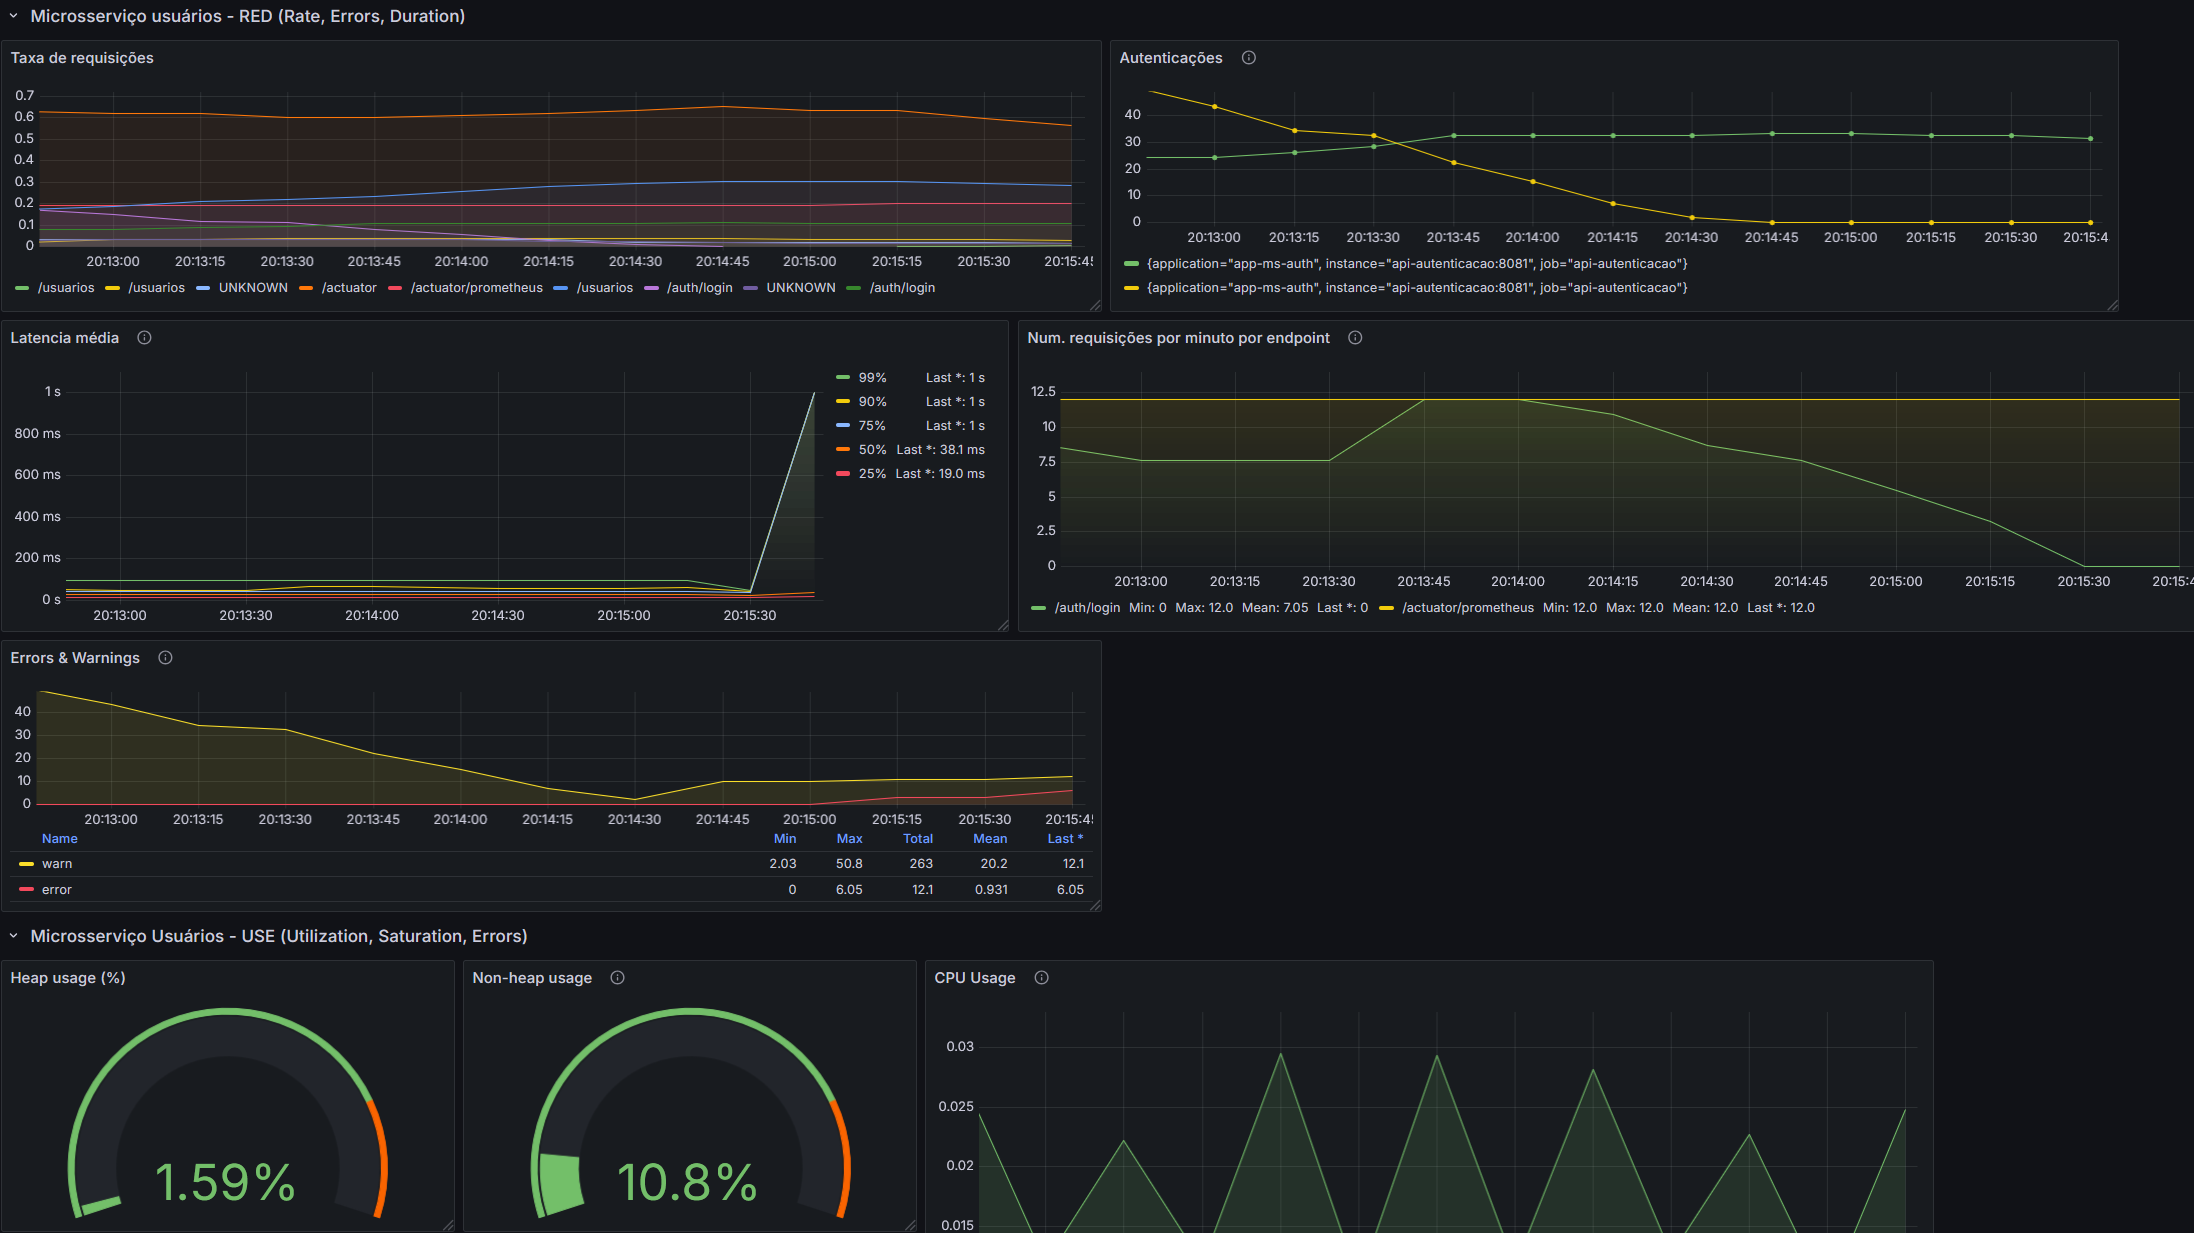
\includegraphics[scale=0.4]{Imagens/dashboard.png}
	\end{center}
	\legend{Fonte: Autor}
\end{figure}

Ademais, também foi implementado \emph{logging} no API \emph{gateway}, usando a funcionalidade embutida do Nginx que grava \emph{logs} no sistema de arquivos com informações de origem da requisição, recurso solicitado, agente usado, entre outros, assim provendo informações de todas as requisições que passam por ele.

\subsection{Padrões de projeto}
O uso de uma arquitetura de microsserviços bem dividida facilita a aplicação de padrões organizacionais, com alguns emergindo naturalmente. Dessa forma, a aplicação obedece a alguns padrões de projeto, citados a seguir.

\subsubsection*{MVC}
Na aplicação exemplar, foi utilizado o padrão MVC (\emph{Model-View-Controller}) sempre que aplicável para organizar a estrutura dos pacotes de forma clara e modular. Devido à divisão natural do tipo de arquitetura tratado, nem todo microsserviço possui essas 3 camadas; nos microsserviços de negócio, por exemplo, não existe a camada \emph{View}. Assim sendo, a divisão foi feita da maneira aplicável a cada microsserviço, garantindo que as responsabilidades fossem bem definidas e que alterações em uma camada não afetassem as demais. Essa divisão também pode ser visualizada no diagrama de pacotes da aplicação.

% Essa abordagem permitiu separar a lógica de negócio (\emph{Model}), a apresentação dos dados (\emph{View}) e o controle do fluxo de execução (\emph{Controller}), facilitando a manutenção e evolução do código. 
\subsubsection*{SOLID}
% \subsubsection*{Orientação a objetos}
Apesar de nem todos os microsserviços usarem exclusivamente o \emph{design} orientado a objetos (JavaScript, por exemplo, é multi-paradigma, mas tem uma tendência para uma abordagem mais funcional), os princípios SOLID também foram adotados no desenvolvimento da aplicação, assim prezando para que cada módulo tivesse apenas uma responsabilidade, que o sistema fosse extensível sem a necessidade de grandes alterações e que as abstrações fossem priorizadas sobre as implementações concretas.
% cada classe e módulo (1) tenham uma única responsabilidade, (2) sejam expandíveis, (3) herdem apenas classes adequadas, (4) implementem apenas interfaces apropriadas e (5) tenham dependências injetadas automaticamente. 

O acesso ao banco de dados em memória no microsserviço de loja, por exemplo, foi encapsulado em uma classe genérica que implementa as funções específicas do banco de dados usado, assim podendo ser substituido por outro com a necessidade apenas de alterar a configuração do banco de dados e a lógica contida dentro dessa classe encapsuladora. Além disso, a dependência dessa classe é injetada diretamente no controlador que a usará, assim seguindo o princípio da inversão da dependência.
% a lógica exclusiva ao banco de dados específico (memcached) dentro de classe que encapsula suas funções específicas 

% Com a aplicação dos princípios SOLID, Essa prática não só promoveu um código mais limpo e modular, mas também facilitou a realização de testes unitários e a manutenção a longo prazo da solução.

\subsubsection*{CLEAN}
Também foram implementados alguns princípios da arquitetura CLEAN, o que favoreceu ainda mais a independência entre os componentes e camadas do sistema. Ao aplicar esse padrão, foi possível isolar a lógica de domínio das dependências externas, como \emph{frameworks} e bancos de dados. Essa separação resultou em um design mais robusto, onde a lógica de negócio permanece centralizada e facilmente testável, permitindo a evolução contínua dos microserviços com risco reduzido de efeitos colaterais indesejados.
Nos microsserviços de loja e usuários, por exemplo, é possível alterar o banco de dados usado sem ser necessário alterações no código, apenas na configuração e dependências.

% O monitoramento foi feito apenas para o microsserviço de usuários por falta de tempo, mas todos os microsserviços podem ser configurados para utilizá-los, e novos \emph{dashboards} podem ser criados para monitorá-los

% Também foi criado um dashboard no grafana com diversas informações importantes de métricas e logging, usando a linguagem PromQL para as consultas ao Prometheus e LogQL para o Loki.
